%!TEX program = xelatex
\documentclass[10pt,svgnames,handout]{beamer}

\PassOptionsToClass{svgnames}{xcolor}

\usetheme[progressbar=frametitle]{metropolis}

\metroset{block=fill}

\usepackage{adjustbox}

\usepackage{fontspec}
\setmainfont{Linux Biolinum O}
\setsansfont{Linux Biolinum O}
\setmonofont{Inconsolata}[Scale=MatchLowercase]
\usepackage{listings}


\lstset{%
  basicstyle=\ttfamily\color{mLightBrown},
  upquote=true
}

\hypersetup{
colorlinks=true,
linkcolor=,
urlcolor=mLightGreen
}

\graphicspath{{./figures/}}

\usepackage{appendixnumberbeamer}

\usepackage{booktabs}

% \usepackage{xspace}
% \newcommand{\themename}{\textbf{\textsc{metropolis}}\xspace}

\title{Git better}
\subtitle{Collaborative project management using \emph{Git} and \emph{Github}}
\date{\today}

\author{Matteo Sostero}
\institute{Sant'Anna School of Advanced Studies}
% \titlegraphic{\hfill\includegraphics[height=1.5cm]{logo.pdf}}

\begin{document}

\maketitle

\begin{frame}{Table of contents}
\setbeamertemplate{section in toc}[sections numbered]
\tableofcontents[hideallsubsections]
\end{frame}

\section{Introduction}

\begin{frame}
\frametitle{Let's Git it done!}
    
These slides are a brief primer to Git, and how it can help your workflow.

\bigskip

\centerline{Find these slides at: \url{bit.ly/}}

\bigskip
\pause

References:
\begin{itemize}
  \item \href{https://www.atlassian.com/git/tutorials}{Atlassian tutorial}
  \item \href{https://guides.github.com/}{Github guides}
  \item \href{http://ndpsoftware.com/git-cheatsheet.html}{Git cheatsheet}
  \item \href{https://git-scm.com/book/en/v2}{Git book}
\end{itemize}
\medskip

Troubleshooting:
\begin{itemize}
  \item \href{https://github.com/blog/2019-how-to-undo-almost-anything-with-git}{How to undo (almost) anything with Git}
  \item \href{https://github.com/k88hudson/git-flight-rules/blob/master/README.md}{Git flight rules}
\end{itemize}
\end{frame}



\section{Version control with Git}

\begin{frame}
\frametitle{Git}

\includegraphics[height=1cm]{Git-logo}

Git is a distributed version control system for tracking changes in files and coordinating work on those files among multiple people.

\textbf{Version control} (Git, Mercurial, CVS, Subversion, Bitkeeper):
\begin{itemize}
   \item keep track of changes to a set of (text, binary) files over time locally;
   \item easily track what changed between any two versions (text);
   \item revert any change if needed;
   \item back up and distribute copies of files;
   \item collaborate on projects.
 \end{itemize} 

\textbf{Distributed}:
\begin{itemize}
  \item developers keep local copy of entire code and history;
  \item can make changes offline and asynchronously;
  \item changes (easily) reconciled later.
\end{itemize}
\end{frame}


\begin{frame}
\frametitle{Git pros}

Advantages of Git:
\begin{itemize}
  \item widely used, supported, documented;
  \item online platforms: \href{https://github.com/}{Github}, \href{https://bitbucket.org/}{bitbucket}, \href{https://about.gitlab.com/}{Gitlab};
  \item dektop interfaces: shell, \href{https://desktop.github.com/}{Github Desktop}, \href{https://www.sourcetreeapp.com/}{SourceTree}, \href{https://www.gitkraken.com/}{GitKraken};
  \item integration in editors and IDEs: Emacs, Sublime Text, RStudio, XCode, Visual Studio, \ldots;
  \item distributed (asynchronous, offline) development;
  \item easy branching: eg, experimental branches for trying changes);
  \item easily make complex merges.
\end{itemize}
\end{frame}


\begin{frame}
\frametitle{Let's Git on the same page}
\label{git_cons}

Challenges:
\begin{itemize}
  \item steep learning curve;
  \item \hyperlink{xkcd_git}{complex conceptual model};
  \item cryptic man pages (but good documentation!).
  \item trivial handling of binary files, images, Office documents;
\end{itemize}

\medskip

Requires some workflow changes (\hypertarget{style}{see details}):
\begin{itemize}
  \item keep project under single directory (\emph{outside} Dropbox, Google Drive, piCloud, \ldots!)
  \item consistency in personal and team coding style (eg, indentation, spacing, line-breaking);
  \item save and commit changes manually and frequently;
  \item requires to document code and explain changes.
\end{itemize}
\end{frame}


\section{Essential concepts}
\begin{frame}
\frametitle{Git concepts: What}
    
\begin{itemize}[<+->]
\item \textbf{repository} (\textbf{repo}): a collection of files and their history:
\begin{itemize}
   \item where the code is kept: under a single root directory;
   \item can be \textbf{local} (your machine), or distributed across your team or on a \textbf{remote} server (eg, Github).
 \end{itemize}

\item \textbf{commit}: a snapshot of your files at a given time:
\begin{itemize}
  \item how Git keeps track of changes in code over time and across team;
  \item manually \textbf{add} one or more files to include to commit them and describe what changed in a message;
  \item a permanent record of what changed (\textbf{diff}), when, by whom, with respect to what (\textbf{parent commit}). Commits are uniquely identified by a SHA-1 code (eg, \texttt{a12b34\ldots});
  \item a repository is “just a directed acyclic graph of commits”.
\end{itemize}
\end{itemize}
\end{frame}

\begin{frame}
\frametitle{Git concepts: Where}

Git has a sophisticated model of \emph{where} things happen, based on how frequently you change things:

\begin{itemize}
\item \textbf{Working directory} (\textbf{working tree, workspace}): the files and sub-directories you can see and work on.\\
\emph{These are visible files stored on your disk.}
\smallskip

\item \textbf{Staging area} (\textbf{index}): where you list files that will go into your next commit.\\
\emph{This is a file in the hidden \texttt{.git/} subdirectory on your disk.}\smallskip

\item \textbf{(local) Repository}: where the commits are stored; ie, it contains the full history of previous versions of the files in the repository, and relevant metadata.\\
\emph{Contained in the hidden \texttt{.git/} subdirectory on your disk.}
\smallskip

\item \textbf{(remote) Repository}: a version of the repository hosted elsewhere.\\
\emph{On another computer, or online service like GitHub or Bitbucket.}
\end{itemize}
\end{frame}


\begin{frame}
\frametitle{Life cycle of files in a repository: from changes to staging area}
\begin{centering}
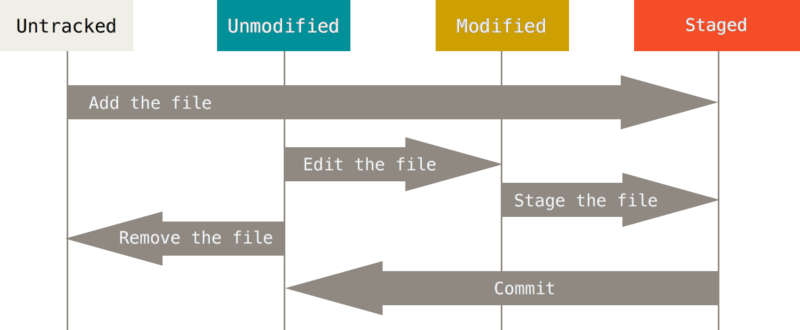
\includegraphics[width=\linewidth]{figures/lifecycle.png}
\end{centering}
\end{frame}


\begin{frame}
\frametitle{Key commands: repository actions}

\begin{itemize}[<+->]
\item \lstinline{git status} (or interface) tells you the state of your repository:
\begin{itemize}
  \item which files are \textbf{untracked} and not indexed.
  \item which files are \textbf{modified} with respect to the index/staging area;
  \item which files are \textbf{staged} (\textbf{indexed}) and ready to be commited;
\end{itemize}
\item \lstinline|git add| new or modified files to the index.
\item \lstinline|git commit| commits changes in the index.
\bigskip
\item \lstinline{git diff} shows what has changed, wrt index or last commit.
\item \lstinline{git log} shows the history of commits up to this point.
\bigskip
\item \lstinline|git push|: send your local changes to the remote server;
\item \lstinline|git pull| (\lstinline{git fetch}; \lstinline{git merge}): get latest changes from remote.
\bigskip
\item \lstinline|git clone|: copy a remote repository on your machine;
\item \lstinline|git init|: start a new repository in empty directory;
\end{itemize}
\end{frame}


\begin{frame}
\frametitle{Example workflow 1}

\begin{block}{Solitary development, offline, from scratch}
    
\begin{enumerate}
  \item Create a new empty directory on your computer
  \item \lstinline|git init|: create a git repository in the directory
  \item create, edit, and save some \texttt{file.txt} in the directory
  \item \lstinline|git status| shows the file is untracked
  \item \lstinline|git add file.txt| to stage the file
  \item \lstinline|git commit -m "First commit! added file.txt!"|
  \item \lstinline|git status| reports no changes
  \item edit the file again, repeat from step (4).
\end{enumerate}
\end{block}
\end{frame}

%TODO: animate.
\begin{frame}
\frametitle{Working with repositories: from changes to commits}
\input{./figures/git_workflow.fig}\\
\begin{small}
Adapted from \href{https://tex.stackexchange.com/a/70332/14260}{Stackoverflow}. See also \href{http://ndpsoftware.com/git-cheatsheet.html}{ndpsoftware.com/git-cheatsheet.html}
\end{small}

\end{frame}



\section{History and branching}

\begin{frame}
\frametitle{History of the repo with \lstinline{git log}}

\input{./figures/linear_history.fig}

\end{frame}


%% Basics: 
% branching
% tag model versions, release

% Workflow:
% branching for features

%% Collaboration


\section{Collaborative development}
% forking, branching, pull request model
% issue tracking and comment
% project readme and collaboration guide


\section{Undoing anything}


\section{Style}

\begin{frame}
\label{style}
\frametitle{Git with style}

Some matters of style and workflow to collaborate with ease.

\begin{itemize}[<+->]
\item repository as self-contained, dedicated directory of (mostly) code:
\begin{itemize}
  \item include \textbf{all} relevant files in the repo (libraries, dependencies, \ldots);
  \item in your code, refer to dependencies using relative paths: \lstinline{./library/}, \textbf{not} \lstinline{/home/user/project_name/library};
  \item exclude unnecessary files (eg, compilation artifacts, large data, useless binary files) using \texttt{.gitignore} (see \href{https://github.com/github/gitignore}{github.com/github/gitignore}).
  \item keep it \textbf{outside} shared folders of Dropbox, Google Drive, piCloud!
\end{itemize}
\item be \textbf{consistent} in personal and team coding style: indentation/tabs, spacing, character encoding (UTF-8), line-breaking.
\item conform to a \textbf{style guide} for your language (eg, \href{https://google.github.io/styleguide/}{google.github.io/styleguide/});
\item \textbf{commit early and often};
\item \textbf{never commit broken code}! use \href{https://git-scm.com/book/it/v2/Git-Tools-Stashing-and-Cleaning}{\lstinline{git stash}} to save it instead.
\item commit related files together;
\item write meaningful commit messages.
\item tag release (baseline, published) versions of your code with \lstinline{git tag}.
\end{itemize}

\end{frame}

\begin{frame}
\frametitle{Example: A LaTeX repo}


\end{frame}




\begin{frame}[standout]
Thank you!
\end{frame}

\appendix

\begin{frame}
\label{xkcd_git}
\frametitle{XKCD on git \hfill\hyperlink{git_cons}{\beamergotobutton{back}}}

\begin{columns}[T,onlytextwidth]
\column{0.45\textwidth}

\includegraphics[width=\textwidth]{figures/xkcd-git.png}

\column{0.45\textwidth}
\vfill
\emph{If that doesn't fix it, git.txt contains the phone number of a friend of mine who understands git.
Just wait through a few minutes of “It's really pretty simple, just think of branches as\ldots” and eventually you'll learn the commands that will fix everything.
}
\end{columns}

\end{frame}

\end{document}
